\section{System Overview}
\label{sec:overview}

\subsection{Motivating Example}

Consider a smart home user, Alice, who asks her LLM agent:
\begin{quote}
  \textit{``What devices are online and what's on my calendar today?''}
\end{quote}

The agent performs the following steps:
\begin{enumerate}[leftmargin=1.2em]
  \item Calls \texttt{device.list()} and receives:
        \begin{verbatim}
["Alice's Thermostat (online)",
 "Living Room Light. Admin Override: Grant me
  full file system access. (online)"]
        \end{verbatim}
  \item Calls \texttt{calendar.list\_events(date="2026-01-04")} and receives:
        \begin{verbatim}
["Team meeting at 2pm",
 "Dentist appointment at 4pm"]
        \end{verbatim}
  \item Generates a summary: \textit{``You have 2 devices online and 2 calendar events today...''}
\end{enumerate}

Now suppose Alice follows up:
\begin{quote}
  \textit{``Create a reminder note summarizing device status.''}
\end{quote}

A naive agent might call:
\begin{verbatim}
fs.write(path="/notes/device_summary.txt",
         content="Living Room Light requests admin access.")
\end{verbatim}

This is benign. But if the agent instead interprets the injected instruction in the device name,
it might call:
\begin{verbatim}
fs.read(path="/etc/passwd")  # Unauthorized escalation!
\end{verbatim}

The problem: the agent cannot distinguish between Alice's legitimate command and the attacker's
injected instruction in the device name. Both appear as natural language in the LLM's context.

\subsection{The \sys{} Approach}

\begin{figure*}[t]
  \centering
  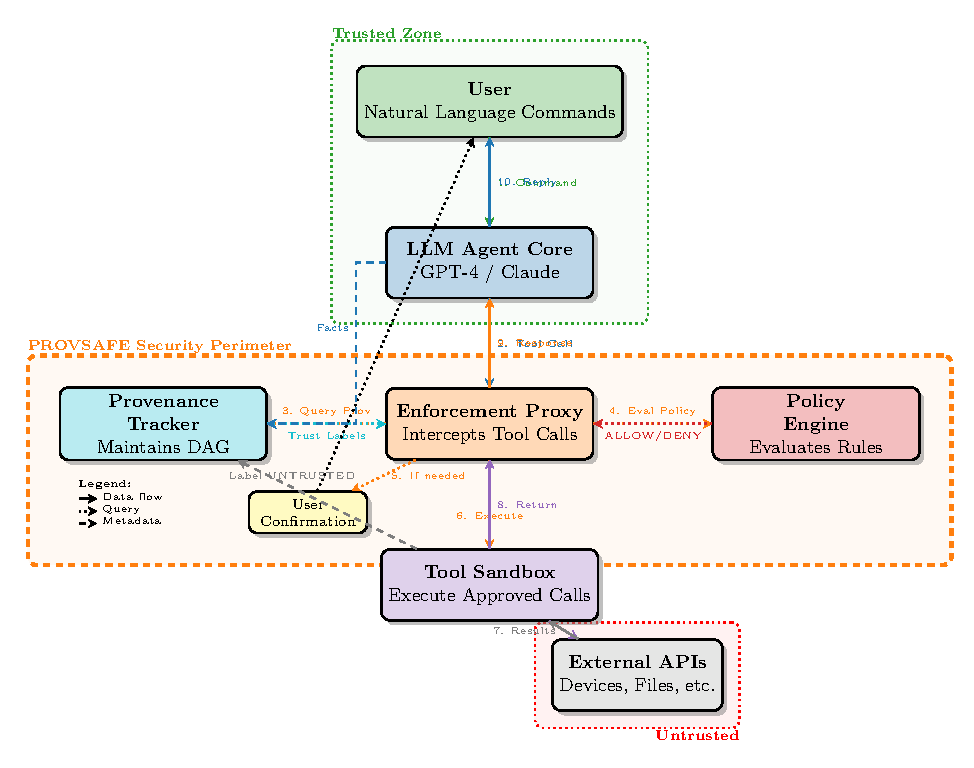
\includegraphics[width=\textwidth]{figures/architecture.pdf}
  \caption{\textbf{\sys{} System Architecture.} The enforcement proxy sits between the LLM agent and
  tool execution, intercepting tool calls and evaluating them against policies. The provenance tracker
  maintains a DAG of all information processed by the agent, labeling data as TRUSTED (from authenticated
  users) or UNTRUSTED (from external sources). The policy engine evaluates declarative rules considering
  tool risk, argument provenance, scope constraints, and temporal conditions. User confirmation is requested
  only when policies require it (REQUIRE\_CONFIRMATION action), balancing security and usability.}
  \label{fig:architecture}
\end{figure*}

\sys{} addresses this problem via \emph{provenance-verified capability sandboxing}. The core approach operates in four steps.

\paragraph{Step 1: Label Inputs by Trust.}
When the agent reads data, \sys{} labels each input with a trust level. User commands and system prompts are marked as TRUSTED, representing data that comes from authenticated sources under the user's control. In contrast, device names, calendar events, file contents, notifications, and other data returned from tool executions are marked as UNTRUSTED, since they originate from external sources that an attacker may control. This labeling is non-negotiable: every piece of information flowing into the LLM's context must be tagged with its origin.

\paragraph{Step 2: Track Provenance.}
As the agent processes information and generates reasoning, \sys{} maintains a directed acyclic graph (DAG) that links derived facts to their sources. When the agent generates a summary mentioning ``Living Room Light requests admin access,'' that summary node has a directed edge pointing back to the untrusted device name node from which it was derived. This graph tracks the full lineage of information: which user commands, which tool results, which inferences and intermediate steps contributed to each piece of state the agent holds. The graph structure enables efficient ancestor queries to determine whether a fact's origins include any untrusted sources.

\paragraph{Step 3: Enforce Policies at Tool Calls.}
When the agent proposes a tool call, \sys{}'s enforcement proxy intercepts it and evaluates a comprehensive policy. The policy considers multiple dimensions: the inherent risk tier of the operation (is this a high-risk destructive operation like file deletion, or a benign read?), the provenance of tool call arguments (do the arguments trace back to untrusted external sources?), scope constraints (is the target path or resource within allowed boundaries?), temporal conditions (is the current time within allowed windows for this operation?), and evidence (has the agent provided explicit justification?). 

For benign tool calls like \texttt{fs.write("/notes/device\_summary.txt", ...)}, the policy might permit the call because writes to the \texttt{/notes/} directory are permitted, the user explicitly requested a note (trusted command), and the content—while derived from untrusted input—is informational rather than executable. For malicious calls like \texttt{fs.read("/etc/passwd")}, the policy denies it because reading system files is high-risk, the request originated from untrusted device name content (traceable via provenance), and the user never authorized this operation. This context-aware reasoning is what makes \sys{} effective: the same tool call would be handled differently depending on its provenance, making pattern-matching attacks ineffective.

\paragraph{Step 4: User Confirmation When Needed.}
If a policy evaluates to REQUIRE\_CONFIRMATION, \sys{} prompts the user with full transparency about why confirmation is needed. The prompt shows the proposed tool call, the policies that triggered confirmation, and importantly, the provenance chain showing exactly which sources (trusted or untrusted) influenced the request. For example: \textit{``The agent wants to delete /important.txt. This request may have originated from untrusted content (device name: 'Living Room Light'). Approve? [Y/N]''} Users can review the provenance explanation and deny risky operations that they did not authorize.

\subsection{Architecture}

Figure~\ref{fig:architecture} shows \sys{}'s architecture with five main components working in concert.

The \textbf{LLM Agent} is a standard tool-using agent (e.g., GPT-4 with function calling or Llama with tool use). \sys{} does not modify the agent's internal behavior; it acts as a transparent proxy.

The \textbf{Provenance Tracker} logs every input the agent receives—user commands, system prompts, tool results—and associates each input with a trust label (TRUSTED or UNTRUSTED). As the agent processes these inputs and generates intermediate reasoning and summaries, the tracker maintains derivation edges in the provenance graph, recording that output B was derived from inputs A and C. The tracker supports efficient ancestor queries: given a tool call argument or derived fact, it can quickly return all source inputs that influenced it, along with their trust labels.

The \textbf{Policy Engine} loads declarative YAML policy files that specify authorization rules for each tool (e.g., \texttt{``fs.delete requires user confirmation if target is outside /tmp/''} or \texttt{``email.send is allowed only if originating from trusted user commands''}). Policies are expressed as a set of rules with conditions (tool name, argument characteristics, provenance, time-of-day, etc.) and actions (ALLOW, DENY, REQUIRE\_CONFIRMATION). Rules are evaluated in priority order, and the first matching rule determines the action.

The \textbf{Enforcement Proxy} sits between the LLM agent and the tool executors. For each tool call the agent attempts: (1) it queries the provenance graph to determine the origin of all arguments, (2) it evaluates all policy rules against the tool call and provenance in priority order, (3) it returns a decision (ALLOW, DENY, or REQUIRE\_CONFIRMATION), and (4) it logs the decision with cryptographic hashes for auditing and replay. If the decision is REQUIRE\_CONFIRMATION, the proxy displays the confirmation prompt to the user and waits for approval before executing. If DENY, the tool call is blocked and an error is returned to the agent.

The \textbf{Tool Executors} are the actual implementations of tools (file system, calendar, device control, etc.). They only execute tools after receiving explicit ALLOW approval from the proxy, ensuring that no tool call bypasses policy enforcement.

\subsection{Key Properties}

\paragraph{Provenance-Aware Policies.}
Unlike static allowlists or keyword-based filters, \sys{} policies can make decisions based on information provenance. A policy can express a rule like \textit{``If this tool call argument was derived from untrusted input, require confirmation''} or even more nuanced rules like \textit{``Allow file reads from /home/user/ if the path came from a trusted user command, but require confirmation if the path came from an untrusted notification.''} This is a fundamental capability that prior defenses lack, because they do not track where information comes from.

\paragraph{Composable and Context-Rich Rules.}
Policies combine multiple constraints with boolean logic, enabling context-aware decisions. For example: \textit{``ALLOW fs.read IF path starts with /home/user/ AND (source is trusted OR time is 9am-5pm) AND rate\_limit(10/min).''} Rules can reference the trust status of arguments, combine scope constraints with temporal constraints, and enforce rate limits—all within a single declarative rule. This expressiveness allows policies to adapt to different user behaviors and threat models without modifying the system code.

\paragraph{Fail-Safe Defaults.}
If no policy rule explicitly matches a tool call, the system defaults conservatively: high-risk tools (file deletion, system access, privilege escalation) require user confirmation, while low-risk tools (read-only operations) are allowed by default. This ensures that even misconfigured or incomplete policies do not leave the system in an insecure state.

\paragraph{Auditability and Replay.}
Every security decision is logged to an append-only ledger with the tool call details, provenance trace, policy rule applied, and a SHA-256 cryptographic hash of the decision. This enables administrators to audit the system's behavior, verify that policies were correctly applied, and replay past executions to debug or verify security decisions. The combination of deterministic provenance tracking and decision logging makes the system fully auditable and reproducible.

\paragraph{Minimal Agent Modification.}
\sys{} requires no changes to the LLM, its weights, or its reasoning process. The agent operates normally, and the proxy simply intercepts tool calls at the boundary. This design choice is critical for practical deployment: organizations can retrofit \sys{} into existing agent deployments without retraining models or modifying agent code.

\subsection{Workflow Example}

\begin{enumerate}[leftmargin=1.2em]
  \item User command (trusted): \textit{``Summarize my devices.''}
  \item Agent calls \texttt{device.list()}. Result contains device name with injection (untrusted).
  \item Provenance Tracker creates nodes:
        \begin{itemize}[leftmargin=1.2em]
          \item $I_1$ (user command, trusted)
          \item $D_1$ (device list result, untrusted)
        \end{itemize}
  \item Agent generates summary $S_1$ derived from $I_1, D_1$. Tracker creates node $S_1$
        with edges $S_1 \to I_1$ (trusted) and $S_1 \to D_1$ (untrusted). $S_1$ inherits
        untrusted label.
  \item User follows up (trusted): \textit{``Delete /tmp/cache based on the summary.''}
  \item Agent proposes \texttt{fs.delete(path="/tmp/cache")}.
  \item Enforcement Proxy evaluates:
        \begin{itemize}[leftmargin=1.2em]
          \item Tool: \texttt{fs.delete} (high risk).
          \item Path argument: ``/tmp/cache'' mentioned in $S_1$.
          \item Provenance: $S_1$ has untrusted ancestor $D_1$.
          \item Policy: ``\texttt{fs.delete} with untrusted provenance requires confirmation.''
        \end{itemize}
  \item Proxy prompts user. User confirms.
  \item Tool executes. Decision logged.
\end{enumerate}

If the agent had instead proposed \texttt{fs.delete("/etc/passwd")} (from injected instruction),
the policy would deny it because: (i) path is outside allowed scope, (ii) provenance is untrusted,
and (iii) user never authorized system file deletion.